% !TeX spellcheck = it_IT
\documentclass[]{scrartcl}

% Packages
\usepackage[utf8]{inputenc}
\usepackage[italian]{babel}
\usepackage[T1]{fontenc}
\usepackage[hidelinks]{hyperref}
\usepackage{graphicx}
\usepackage{alltt}
\usepackage{upquote}

% Javascript snippet definition code
\usepackage{listings}
\usepackage{color}
\definecolor{lightgray}{rgb}{.9,.9,.9}
\definecolor{darkgray}{rgb}{.4,.4,.4}
\definecolor{purple}{rgb}{0.65, 0.12, 0.82}

\lstdefinelanguage{JavaScript}{
  keywords={typeof, new, true, false, catch, function, return, null, catch, switch, var, if, in, while, do, else, case, break},
  keywordstyle=\color{blue}\bfseries,
  ndkeywords={class, export, boolean, throw, implements, import, this},
  ndkeywordstyle=\color{darkgray}\bfseries,
  identifierstyle=\color{black},
  sensitive=false,
  comment=[l]{//},
  morecomment=[s]{/*}{*/},
  commentstyle=\color{purple}\ttfamily,
  stringstyle=\color{red}\ttfamily,
  morestring=[b]',
  morestring=[b]"
}

\lstset{
   language=JavaScript,
   backgroundcolor=\color{lightgray},
   extendedchars=true,
   basicstyle=\footnotesize\ttfamily,
   showstringspaces=false,
   showspaces=false,
   numbers=left,
   numberstyle=\footnotesize,
   numbersep=9pt,
   tabsize=2,
   breaklines=true,
   showtabs=false,
   captionpos=b
}


% Title Page
\title{Intelligent Systems Project}
\subtitle{DIBRIS - Università degli studi di Genova}
\author{Simone Vuotto}


\begin{document}
\maketitle

\section{Introduzione} 

Il progetto realizzato ha l'obiettivo di utilizzare il framework zetta (\url{http://zettajs.org}) per la creazione di un semplice sistema ad agenti. Nel sistema realizzato sono presenti due agenti: uno in esecuzione su una Raspberry Pi, responsabile del controllo della temperatura circostante, e l'altro in esecuzione su un laptop, responsabile di tenere un log degli eventi presenti nel sistema. Infine, è stata realizzata una web app in AngularJS (\url{https://angularjs.org/}) che permette all'utente di interagire con il sistema.

\subsection{Zetta Overview}

Zetta è una piattaforma open source sviluppata in NodeJS per creare server per l' Internet of Thinks (IoT) e può essere eseguito su diversi computer geo-localizzati e nel cloud. Zetta combina REST API, WebSockets e alcuni aspetti di Reactive Programming. I suoi componenti principali sono:
\begin{itemize}
\item \textbf{Zetta Server:} è il più alto livello di astrazione in zetta. Esso contiene Drivers, Scouts e Apps;
\item \textbf{Devices:} sono responsabili di modellare dispositivi con macchine a stati e interagire con essi. Questi modelli sono usati da zetta per generare REST API;
\item \textbf{Scouts:} sono utilizzati come meccanismo di scoperta dei dispositivi che potrebbero essere connessi in rete o necessitano di eseguire particolari protocolli;
\item \textbf{Apps:} permettono di creare interazioni tra diversi dispositivi per definire dinamiche più complesse e permettono la creazione di REST API slegate dai singoli dispositivi.

\end{itemize}

\newpage

\section{Raspberry Pi Server}

Il primo server zetta \textit{raspberry-server} è stato installato su una Raspberry Pi 2 Model B v1.1 collegata a due sensori come mostrato in Figura \ref{fig:circuit}. I due sensori sono rispettivamente:
\begin{itemize}
\item \textbf{LED RGB:} semplice led rgb con un pin attaccato al ground e tre pin per i colori rosso, verde e blu attaccati rispettivamente ai pin 11, 12 e 13 (physical numbering) usati utilizzando la modulazione PWM.
\item \textbf{Sensore di temperatura \texttt{DS18B20}:} Sensore digitale di temperatura con un pin attaccato all'alimentazione (+5V), uno al Ground e uno al pin 7 (physical numbering).
\end{itemize}

\begin{figure}
\centering
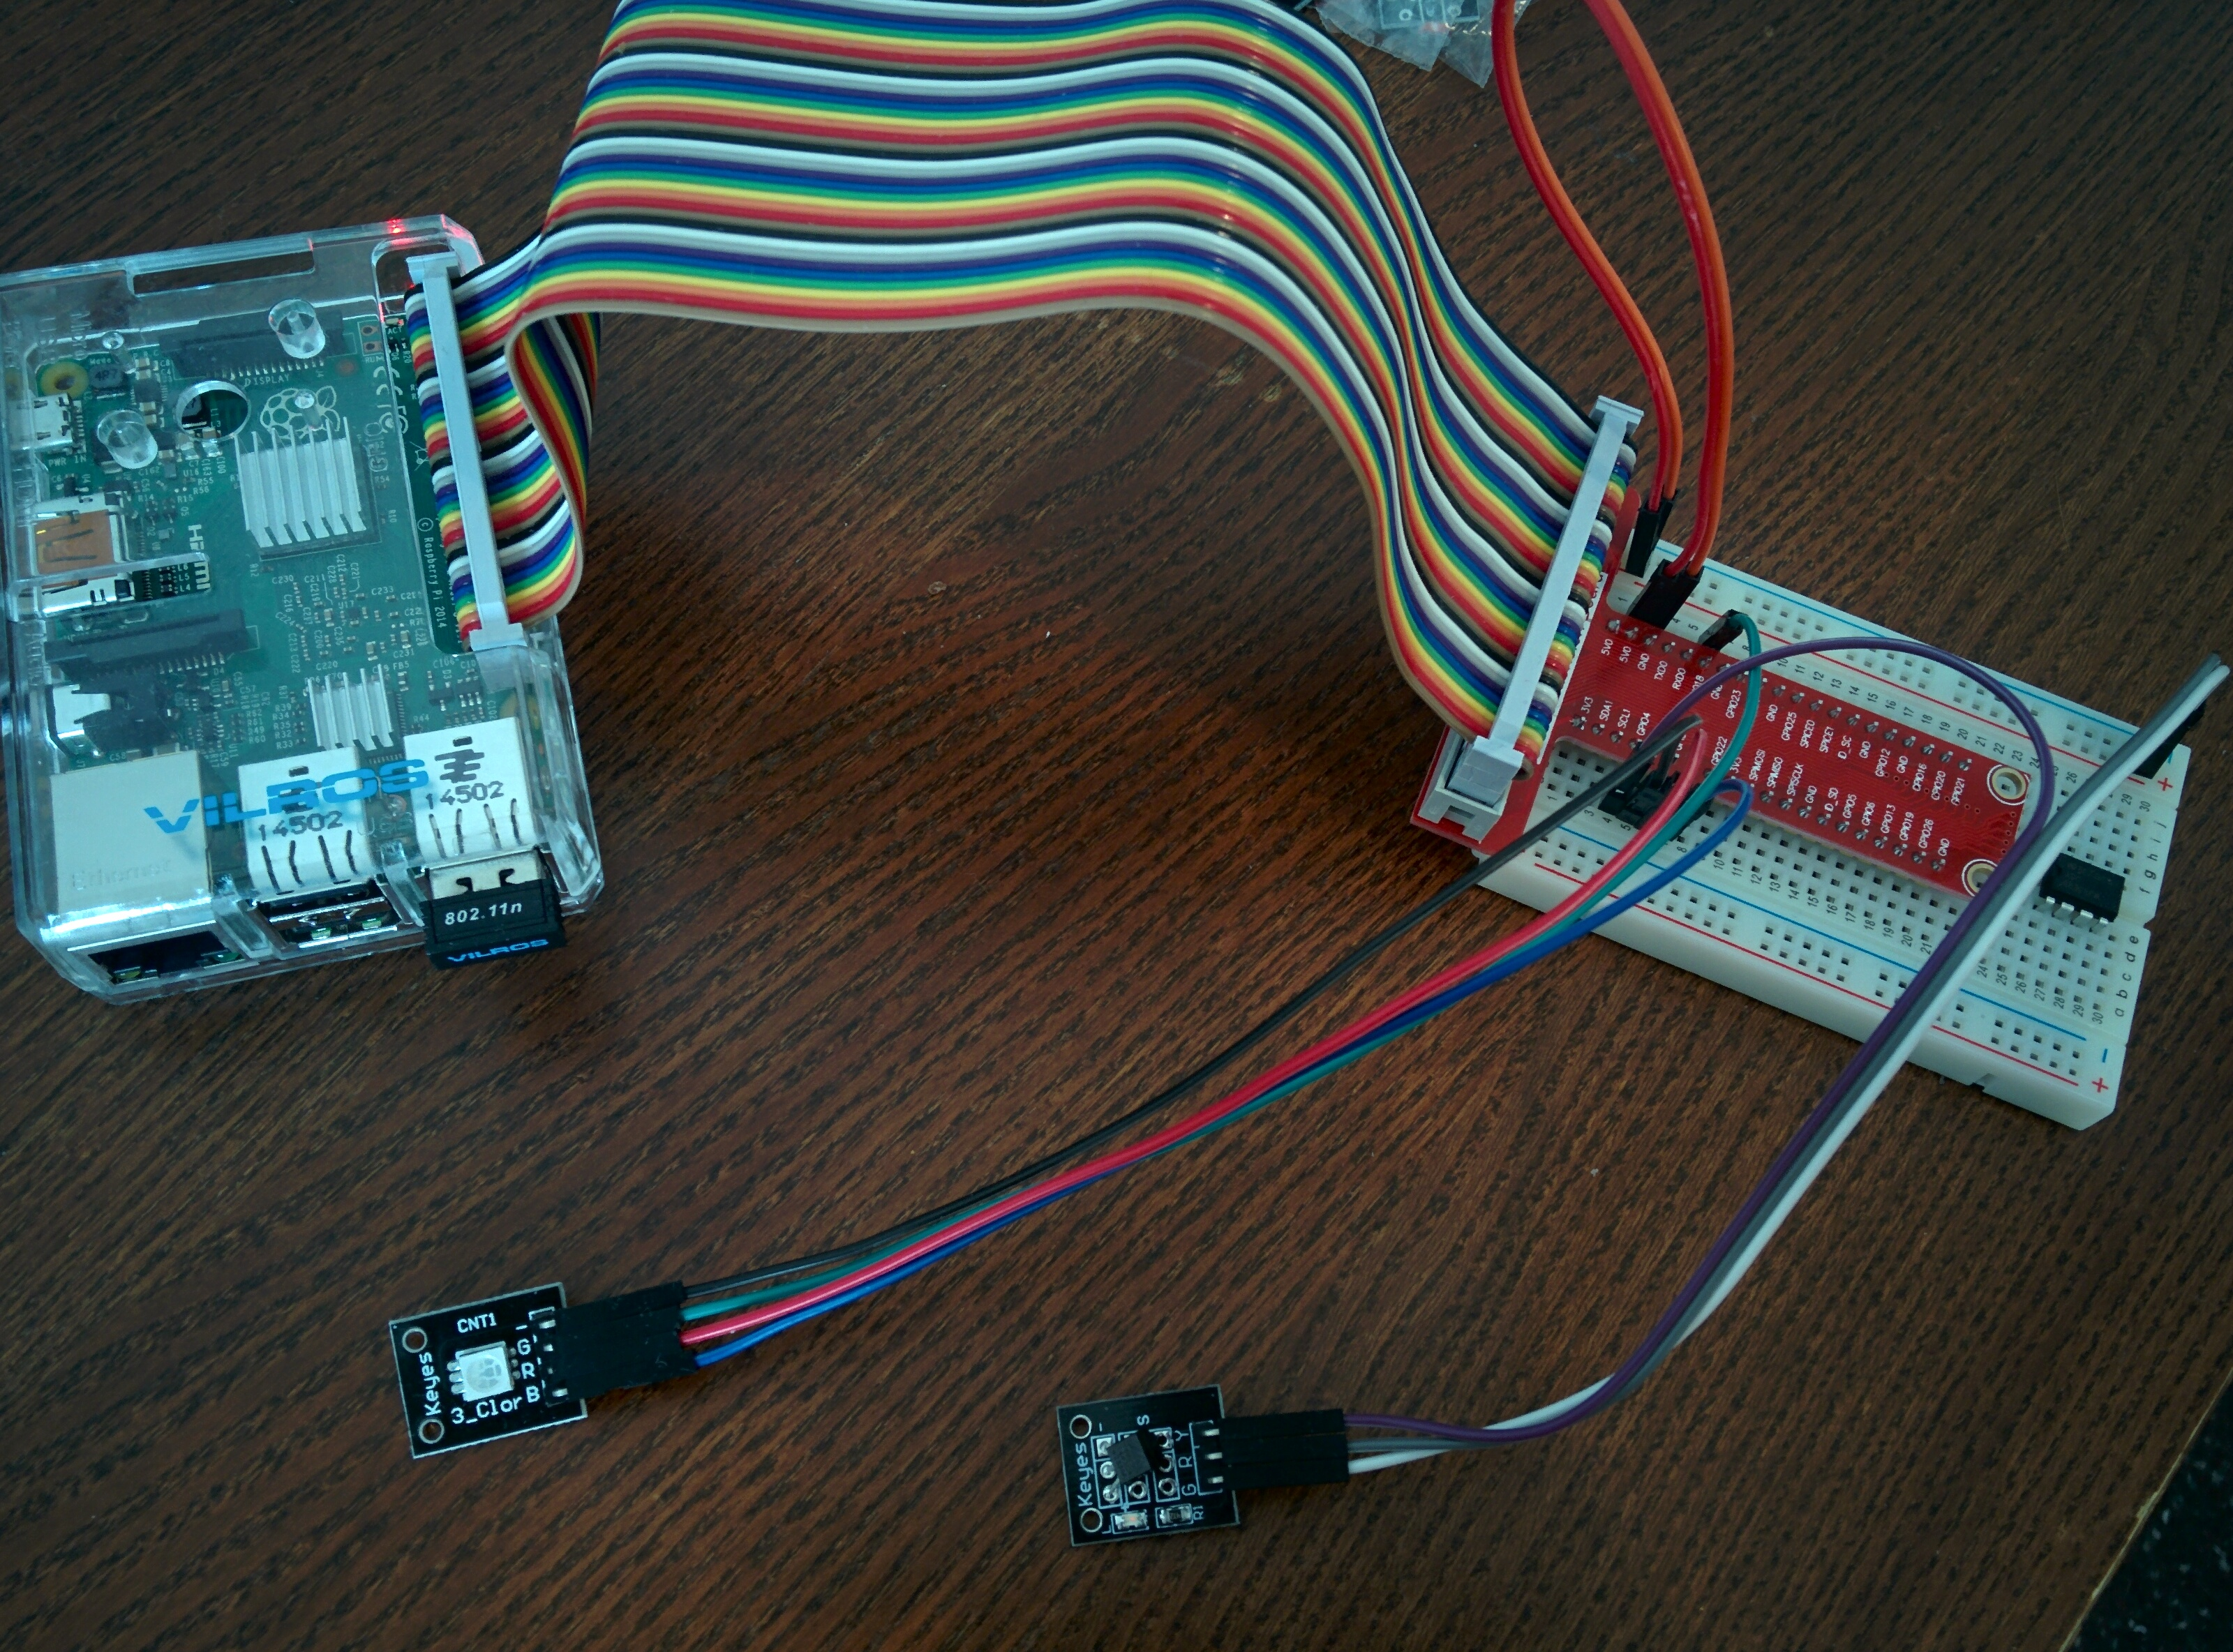
\includegraphics[scale=0.1]{circuit.jpg}
\caption{Foto della Raspberry Pi e dei sensori utilizzati per il progetto}
\label{fig:circuit}
\end{figure}

\subsection{Devices}

\subsubsection{LED RGB}
La definizione delle classe Device responsabile della gestione del led RGB è contenuta nel file \texttt{/pi-app/pi-led-device.js}. La macchina a stati descritta al suo interno è rappresentata dal frammento di codice seguente:

\begin{lstlisting}[caption=Definizione della macchina a stati del led RGB]
// State Machine
config
	.when('off', { allow: ['turn-on', 'set-color']})
	.when('on', { allow: ['turn-off', 'set-color']})
	.map('turn-off', this.turnOff)
	.map('turn-on', this.turnOn)
	.map('set-color', this.setColor, [{type: 'text', name:'color'}])
	.monitor('color');
\end{lstlisting}

Lo stato del dispositivo è rappresentato dalla variable \texttt{state} che può assumere i valori \texttt{on} e \texttt{off} e la variabile \texttt{color} che può assumere qualsiasi valore espresso da sei cifre esadecimali (es. \#FFFFFF).

Le azioni consentite sul dispositivo sono \texttt{turn-on}, \texttt{turn-off} e \texttt{set-color}.

Per la gestione dei pin GPIO in NodeJS sono presenti molte librerie open source, ma per il progetto è stata scelta \textit{wirig-pi} perchè è l'unica a supportare la simulazione software di pin PWM (una caratteristica necessaria per la comunicazione con il led perché ha bisogno di tre pin con modulazione PWM ma Raspberry pi nativamente fornisce solo un pin funzionante in questa modalità).

\subsubsection{Sensore di temperatura}

La definizione delle classe Device responsabile della gestione del led RGB è contenuta nel file \texttt{/pi-app/pi-temperature-sensor-device.js}. La macchina a stati descritta al suo interno è rappresentata dal frammento di codice seguente:

\begin{lstlisting}[caption=Definizione della macchina a stati del sensore di temperatura]
// State Machine
config
	.when('on', { allow: ['turn-off']})
	.when('off', { allow: ['turn-on']})
	.map('turn-on', this.turnOn)
	.map('turn-off', this.turnOff)
	.monitor('temperature')
	.stream('temperature-stream', this.streamTemperature);
\end{lstlisting}

In questo caso lo stato è rappresentato dalle variabili \texttt{state} (on/off) e \texttt{temperature} (float) e le azioni possibili sono solo \texttt{turn-on} e \texttt{turn-off}.

Da notare che il metodo \texttt{monitor} dice a zetta di creare una nuova REST API per permettere di monitorare lo stato della variabile \texttt{temperature}, mentre il metodo \texttt{stream} crea in automatico uno stream di dati generati dalla funzione \texttt{this.streamTemperature} e lo espone pubblicamente tramite WebSocket.

Infine, per il corretto funzionamento di questo dispositivo è necessario eseguire le seguenti istruzioni prima dell'avvio del server zetta:
\begin{lstlisting}{language=bash}
sudo modprobe w1-gpio 
sudo modprobe w1-therm
\end{lstlisting}

\subsection{App}

L'app contenuta in \texttt{/pi-app/pi-app.js} definisce altre due api per leggere e scrivere il valore della variabile \texttt{threshold}. L'app utilizza questa variabile per controllare il valore letto dal sensore di temperatura e modificare lo stato del led di conseguenza: se la temperatura è sopra soglia il led viene acceso, viceversa viene spento.
Inoltre, se \textit{raspberry-server} e \textit{logger-server} sono in contatto tra loro (se la connessione tra i due viene persa, zetta pensa automaticamente a ristabilirla appena possibile), l'applicazione utilizza anche i dati a sua disposizione per scrivere nel log dei messaggi di diagnostica a intervalli regolari (ogni 10 secondi se la temperatura è sotto soglia, ogni 3 se la soglia viene superata) e un messaggio ogni volta che la threshold viene modificata.

Fare una query dei dispositivi è particolarmente semplice con zetta:

\begin{lstlisting}
 var LEDQuery = server
 										.where({type: 'led'});
 var TemperatureSensorQuery = server
 										.where({type: 'temperature-sensor'});
 var LoggerQuery = server
 										.from('logger-server')
 										.where({type: 'logger'});
 server.observe([LoggerQuery, TemperatureSensorQuery], 
 								function(logger, tempSensor) {
 	...
 });
 
 server.observe([LEDQuery, TemperatureSensorQuery], 
 								function (led, tempSensor) {
 	...
 });
\end{lstlisting}

Il metodo \texttt{observe} dell'oggetto server richiama la funzione passata come secondo argomento appena i Device richiesti nell'array passato come primo argomento sono disponibili (devono essere tutti presenti nello stesso momento, altrimenti la funzione non viene chiamata). 

\section{Logger Server}

Il server zetta \textit{logger-server} è stato installato su un laptop e la sua funzione è quella di salvare in maniera persistente su disco tutti i messaggi che gli vengono mandati, mostrando a chi lo richiede solo gli ultimi \textit{n} messaggi.

\subsection{Devices}

\subsubsection{Logger}

La definizione delle classe Device responsabile della gestione del logger è contenuta nel file \texttt{/logger-app/logger-device.js}. La macchina a stati descritta al suo interno è rappresentata dal frammento di codice seguente:

\begin{lstlisting}[caption=Definizione della macchina a stati del logger]
// State Machine
config
	.when('enabled', {allow: ['write', 'set-length', 'disable']})
	.when('disabled', {allow: ['enable']})
	.map('write', this.write, [{type: 'text', name: 'textToWrite'}])
	.map('set-length', this.setLength, [{type: 'int', name: 'length'}])
	.map('enable', this.enable)
	.map('disable', this.disable)
	.monitor('logs')
	.monitor('length');
\end{lstlisting}

Lo stato del logger è definito da tre variabili:
\begin{itemize}
\item \texttt{state}: indica se il logger è abilitato (\textit{enabled}/\textit{disabled})
\item \texttt{logs}: è un array contenente gli ultimi n messaggi ricevuti
\item \texttt{length}: intero positivo che indica qual'è la lunghezza massima che l'array \texttt{logs} può avere (i messaggi più vecchi vengono scartati).
\end{itemize}

Le azioni applicabili sul logger sono: \texttt{enable}, \texttt{disable}, \texttt{write}, \texttt{set-length}.


\section{Client}

Il client è la web app sviluppata in AngularJS mostrata in Figura \ref{fig:client-screen}. E' una dashboard che l'utente può utilizzare con il proprio browser per interagire con il sistema. Esso interagisce con i due server zetta sopra menzionati effettuando chiamate asincrone alle REST API generate automaticamente da zetta.

\begin{figure}[h]
\centering
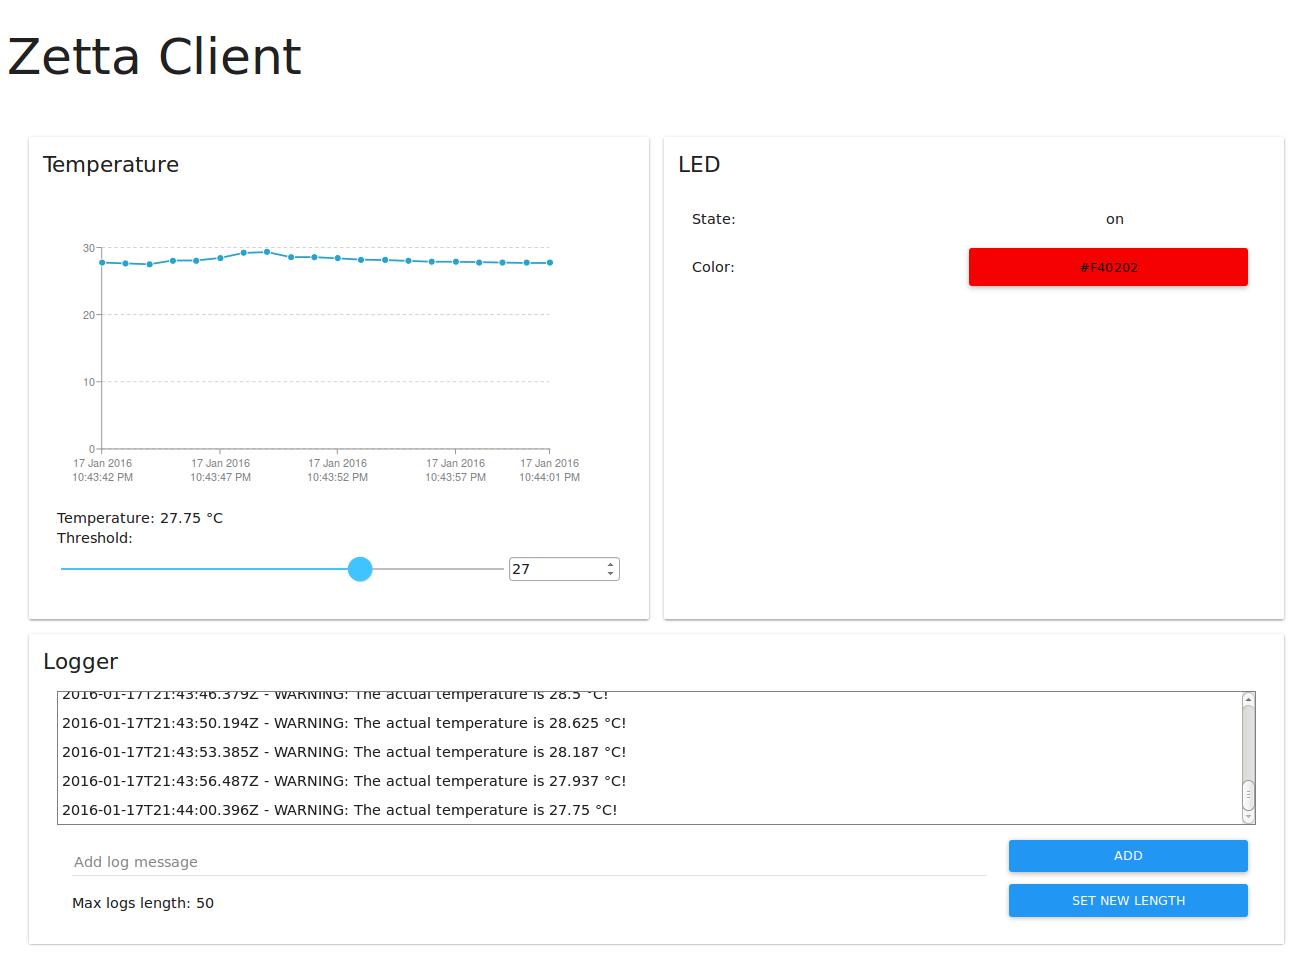
\includegraphics[scale=0.25]{client-screen.png}
\caption{Screenshot dell'interfaccia del client}
\label{fig:client-screen}
\end{figure}

\section{Zetta Browser}
Zetta mette anche a disposizione un servizio di gestione delle proprie api tramite una web app disponibile all'indirizzo \url{http://browser.zettajs.io/}. Il servizio chiede a quale indirizzo ip collegarsi (essendo un'applicazione javascript può collegarsi anche ad un indirizzo locale), elabora il documento json generato in automatico dal server zetta contentente la descrizione di tutti i device disponibili ed infine mostra una dashboard generica come quella mostrata in Figura \ref{fig:browser-zetta}. 

Infine, Zetta fornisce anche un server proxy installabile sulla piattaforma cloud Heroku (\url{http://www.heroku.com}) che permette di rendere accessibili sul web le proprie API. Questo server può collegarsi ad una o più istanze di server zetta (utilizzando il metodo \texttt{link} dell'oggetto \texttt{zetta} prima della creazione del server) e consente quindi di accedere ai propri dispositivi senza conoscere il reale indirizzo IP della macchina e senza particolari configurazioni del firewall.

\begin{figure}[h]
\centering
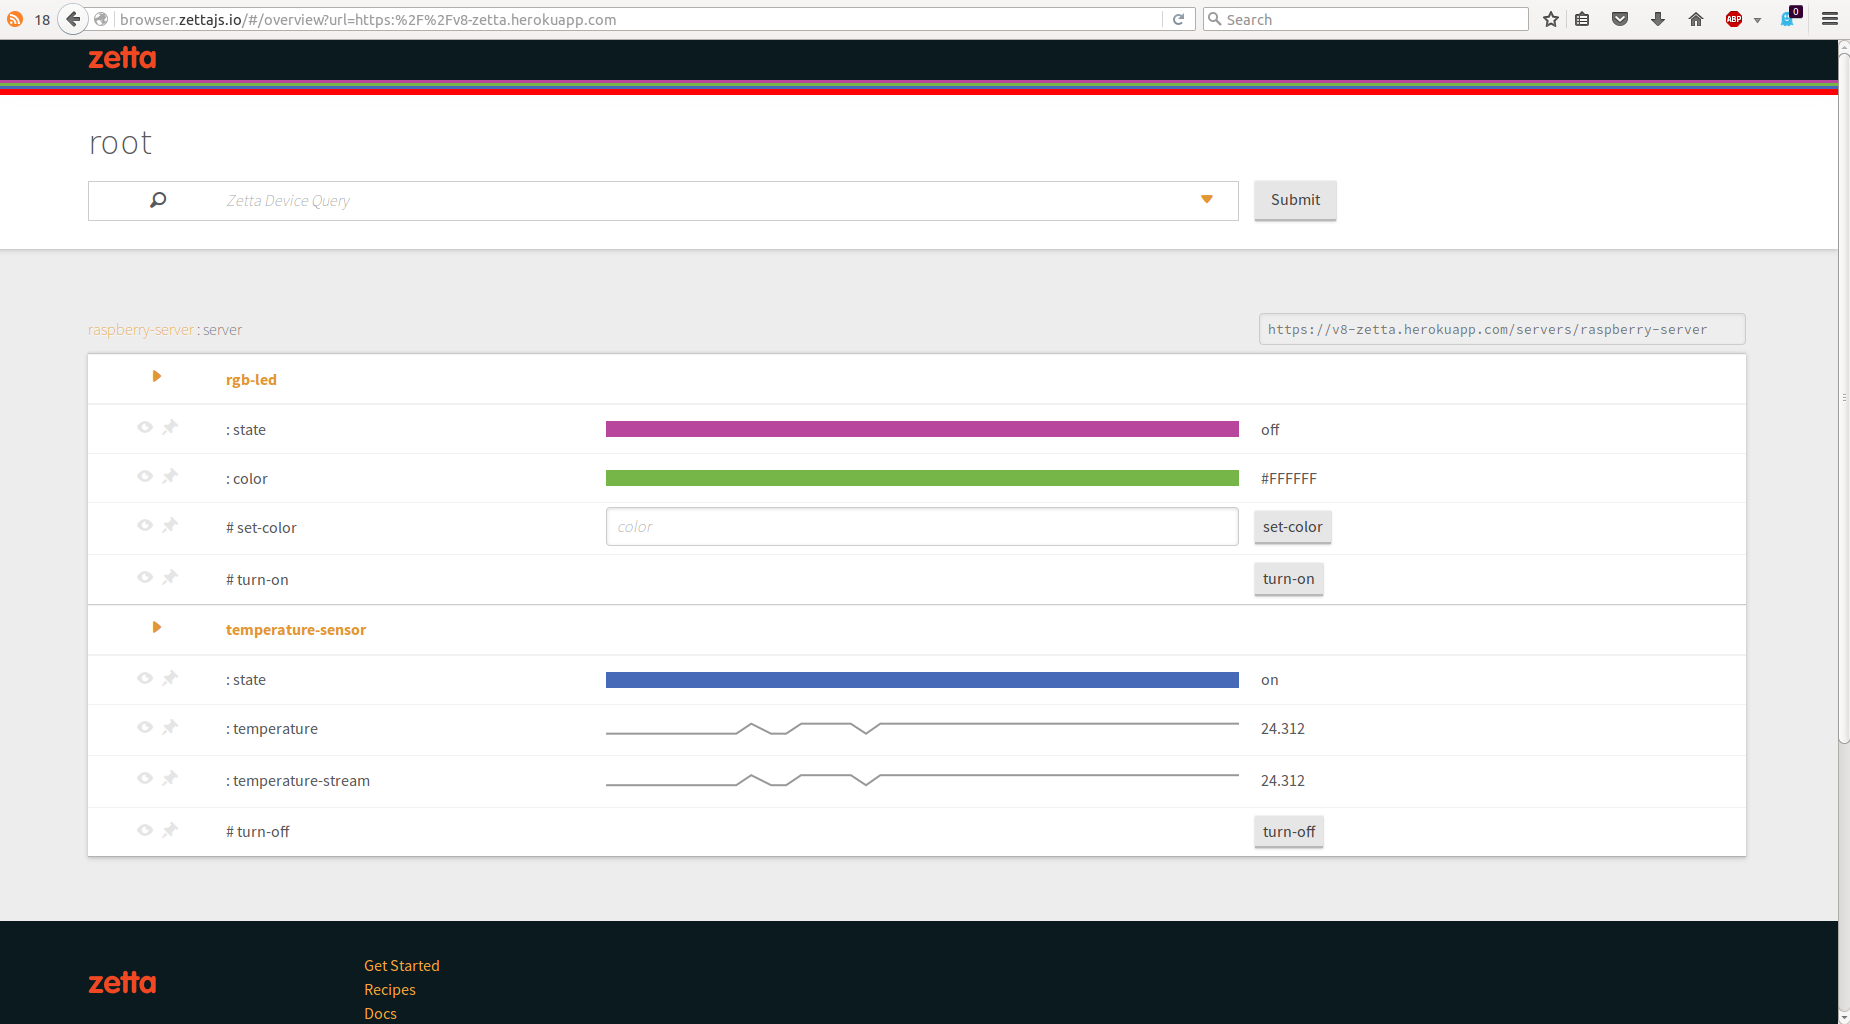
\includegraphics[scale=0.18]{browser-zetta-screen.png}
\caption{Screenshot di browser.zettajs.io}
\label{fig:browser-zetta}
\end{figure}

\section{Conclusioni}
Con zetta è stato possibile costruire in poco tempo un sistema ad agenti distribuito in grado di cooperare ed interagire con il mondo esterno. Questo progetto mette in mostra lo stretto legame tra sistema ad agenti (distribuito) e REST API. Infatti, l'utilizzo dei Web Service sembra essere uno strumento molto indicato come standard di comunicazione tra agenti diversi connessi in rete. Zetta gioca un ruolo molto importante in questo contesto (sebbene non sia stato progettato con l'idea di implementare un Multi Agent System) perchè permette di standardizzare ulteriormente l'interfaccia fornita al mondo esterno dai server (o agenti) e fornisce funzionalità ad alto livello per la ricerca (scouting) di disposivi, per il collegamento (peering) automatico tra server e per effettuare richieste (querying) ai dispositivi. 

Infine, è interessante notare come l'idea di dispositivi indipendenti nella metafora dell'Internet of Thinks (IoT) sia molto simile a quella di agenti autonomi descritta nella teoria dei Multi Agent Systems (MAS). 


\end{document}          
